\chapter{UR5 - Delimited Cobot}

In this chapter the specifications of the delimited cobot will be presented.

\section{UR}

Universal Robots was founded in 2005 by a group of Danish engineers. Their thought was, that every industrial robot on the market was designed to be big, heavy and expensive. Therefore the group decided to make a smaller and more agile kind of industrial robot.\cite{Urhist}\\
Here are the specification for the UR5:\\ 

\subsubsection{UR5}

\begin{itemize}
    \item Weight: 18.4 kg.
    \item Payload: 5 kg.
    \item Footprint: 149 mm.
    \item Joints: +/-360 degrees on all the joints.
    \item Operating life: 35,000 Hours.
    \item Speed: joints = 180 degrees/sec, tool = 1 m/sec.
    \item Reach: 850 mm.
    \item Repeatability: +/- 0.1 mm.
\end{itemize}

The materials used on all the cobots are aluminum and plastic\cite{Ur5_about}\cite{UR5_tech}.\\

\begin{figure}
    \centering
    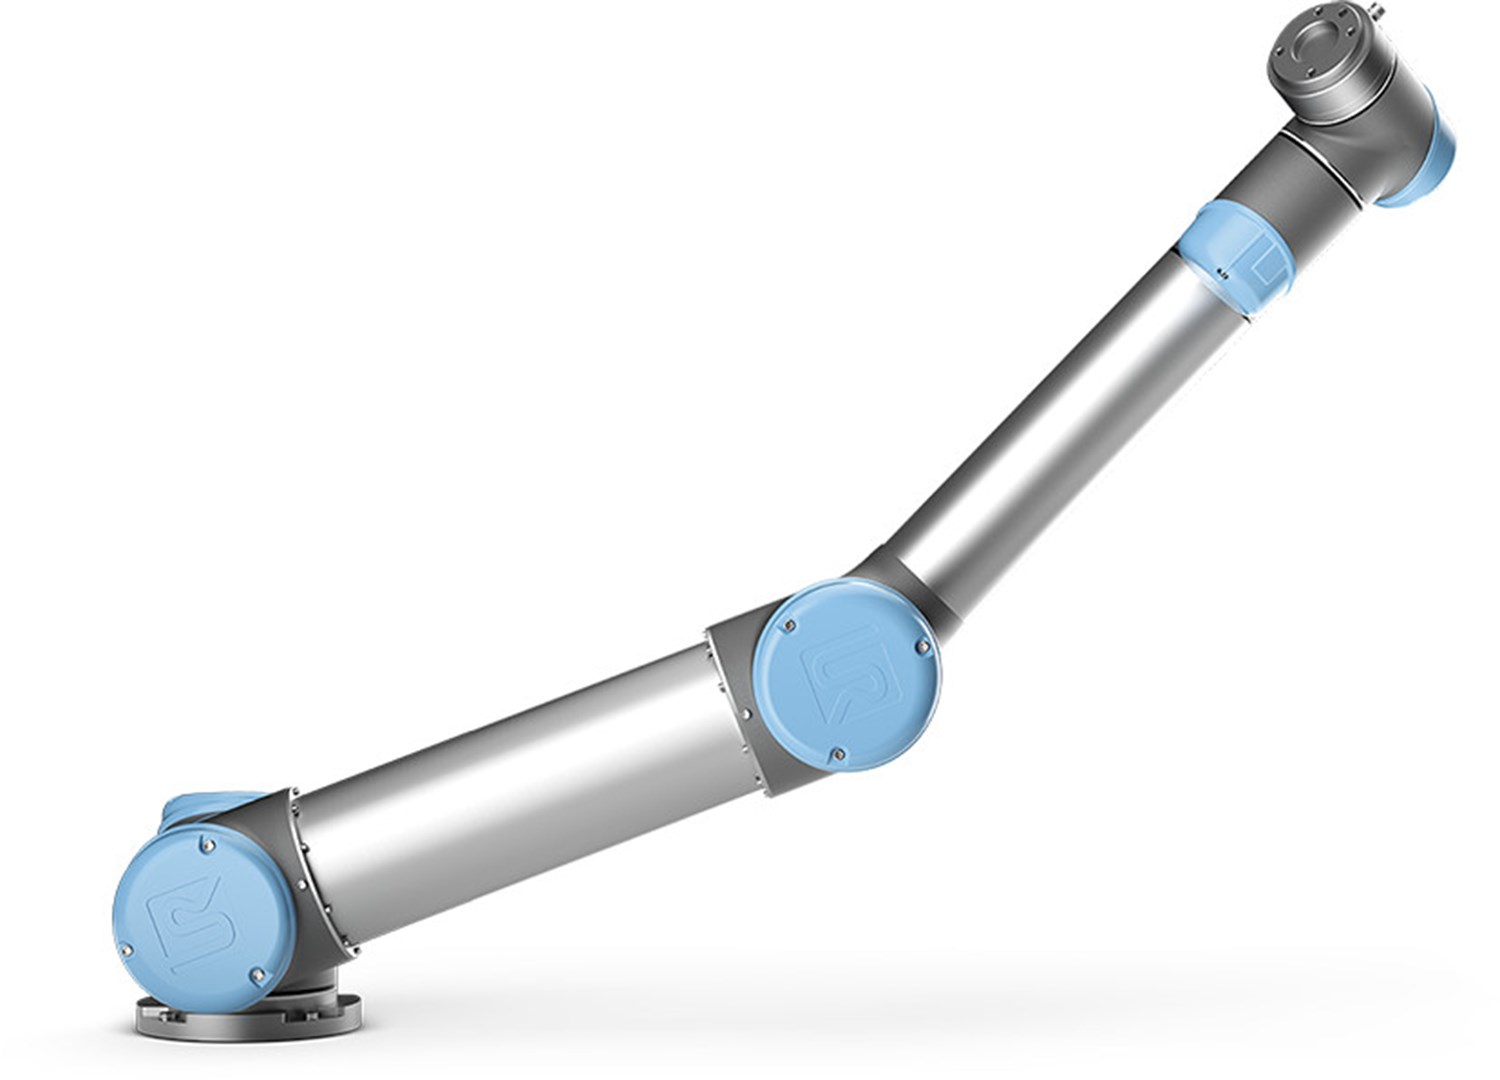
\includegraphics[width=9cm]{UR/UR5pic.jpg}
    \caption{Universal Robots UR5 \cite{UR5billede}}
    \label{fig:UR5}
\end{figure}